V tem podpoglavju bodo predstavljeni rezultati testiranja različnih indeksov besede. Testiranje je bilo izdelano z metodo in računalnikom predstavljenim v podpoglavju \ref{sec:opis}. Meritve lahko ločimo na dva dela, in sicer: meritvi vezani na gradnjo, ki sta čas gradnje in velikost podatkovne strukture, ter poizvedbe z indeksom. Zato bo sledeče podpoglavje tudi razdeljeno na dva dela. V vsakem delu bodo ločeno predstavljeni rezultati testiranja za vsako testno besedo iz Tabele \ref{tab:besedila}. V podpoglavju \ref{sec:razprava} pa bo narejena bolj podrobna razprava o rezultatih testiranja.

Dolžina najdaljše vhodne besed $n_{max}$ je bila sprva nastavljena na 4000000 znakov. Med testiranjem priponskega drevesa besede dolžine 2048000 znakov opazimo, da je čas, potreben za izgradnjo prvega priponskega drevesa, presegal pet minut. V tem trenutku je bil delovni pomnilnik v celoti zaseden ter 6 GB pomnilniških strani je bilo premaknjenih na Swap prostor. Pri tem je bil računalnik neodziven in proces je bil v neprekinjenem spanju (angl. \textit{Uninterruptible sleep} ali stanje D). Na Sliki \ref{fig:6GB} je prikazan upravljalnik opravil Htop v času izgradnje priponskega drevesa za besedo dolžine 2048000 znakov. Proces v modri vrstici predstavlja program za testiranje časa izgradnje in poizvedb ter prostorske zahtevnosti indeksov besed. V stolpcu, označenim S (Stanje ali angl. \textit{Status}), je vidno, da je stanje procesa označeno kot D, ker je proces v neprekinjenem spanju. Po več kot 5 minutah od začetka gradnje priponskega drevesa za besedo dolžine 2048000 znakov smo se odločili, da se proces ubije. Posledično se je znižala velikost besede za izgradnjo zadnjega indeksa na 1024000 znakov. Med testiranjem smo opazili tudi, da se $LCP$ polje ne zgradi za besede dolžine 1024000 znakov in smo se odločil, da se ta test v zadnjem koraku izpusti.

\begin{figure}[tb]
    \centering
    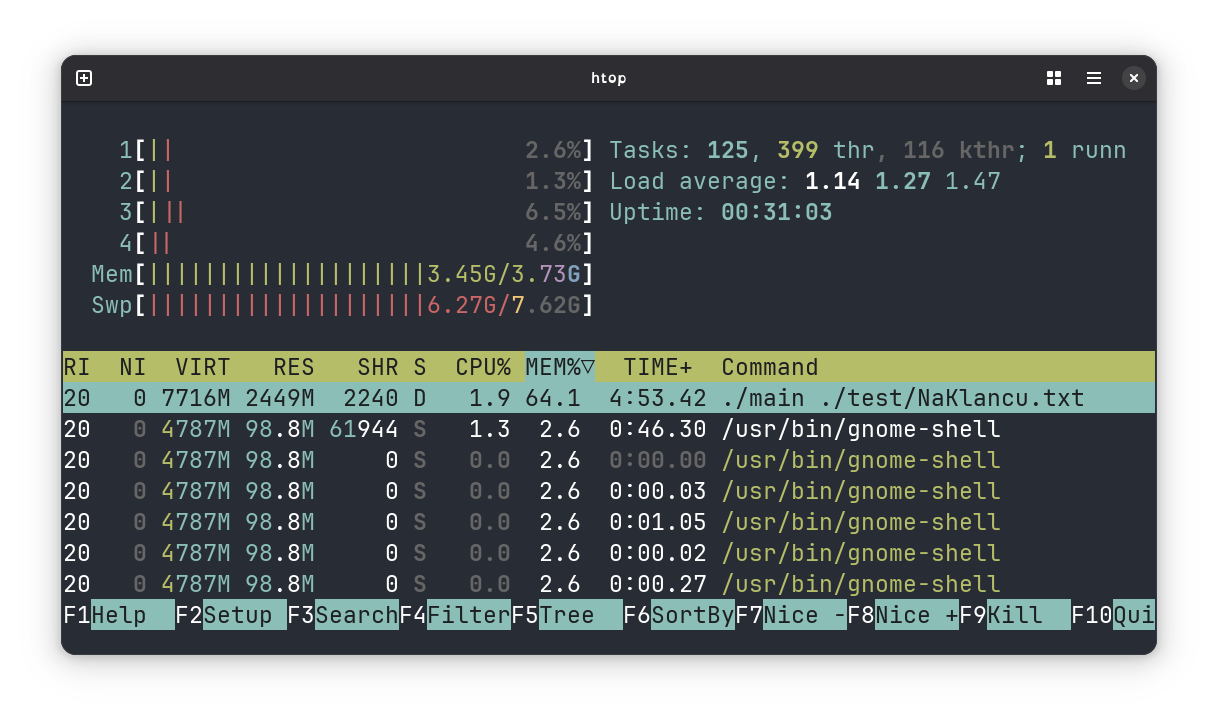
\includegraphics[width=\textwidth]{Slike/Zaslonski posnetek 2025-06-23 22-53-56.png}

    \caption{Posnetek zaslona upravljalnika opravil Htop med izgradnjo priponskega drevesa za besedilo dolžine 2048000 znakov.} 
    \label{fig:6GB}
\end{figure}


\subsection{Gradnja}
Najprej bodo predstavljeni rezultati gradnje. Prvo bodo predstavljeni rezultati meritev velikosti podatkovnih struktur, zatem pa bodo predstavljeni rezultati časov potrebnih za gradnjo.

\paragraph{Velikost podatkovne strukture.}

Rezultati meritve prostorske zahtevnosti so prikazani na Sliki \ref{fig:VelikostGraf} za \DNK\ in na Sliki \ref{fig:VelikostGrafSLO} za \NK. Iz obeh testiranj se vidi, da je prostorska zahtevnost priponskega drevesa večja kot prostorska zahtevnost ostalih indeksov. Pri tem vidimo tudi, da prostorska zahtevnost linearno raste z velikostjo besede, za vse 4 testirane podatkovne strukture.

\begin{figure}[htb]
    \centering
    \includesvg[inkscapelatex=false,width=\textwidth]{Slike/velikostDrecvesaNovPC.svg}
    \caption{Graf velikosti indeksov izgrajenih iz besed različni velikosti. Vhodna beseda je \DNK.} 
    \label{fig:VelikostGraf}
\end{figure}

Iz rezultatov testiranja za \DNK, Slika \ref{fig:VelikostGraf}, vidimo, da priponsko polje (označeno z zeleno barvo), priponsko polje z LCP poljem (označenim z modro barvo) in kompaktno priponsko drevo (označeno z rdečo barvo) potrebujejo bistveno manj prostora, kot ga potrebuje priponsko drevo (označeno z viola barvo).

\begin{figure}[tb]
    \centering
    \includesvg[inkscapelatex=false,width=\textwidth]{Slike/velikostDrecvesaNovPCSLO.svg}
    \caption{Graf velikosti indeksov izgrajenih iz besed različni velikosti. Vhodna beseda je roman \NK.} 
    \label{fig:VelikostGrafSLO}
\end{figure}

Podobno se lahko vidi tudi za \NK, Slika \ref{fig:VelikostGrafSLO}. Velikost vseh podatkovnih struktur linearno raste z dolžino vhodne besede, pri čemer priponsko drevo (označeno z viola barvo) potrebuje bistveno več prostora kot ostale podatkovne strukture. Pri tem pa se vidi, da je razlika v zasedenem prostoru med priponskim drevesom in ostalimi indeksi nižja in približno konstantna skozi celotno izvajanje testa, za razliko od testa nad \DNK.


\paragraph{Čas potreben za gradnjo.} 

Rezultati so prikazani na Sliki \ref{fig:IzgradnjaGraf} za \DNK\ ter na Sliki \ref{fig:IzgradnjaGrafSLO} za \NK. V obeh primerih vidimo, da čas gradnje indeksov raste linearno z dolžino besede. V obeh testnih primerih se priponsko polje (označeno z zeleno barvo) zgradi najhitreje. Iz slik se zdi, da kompaktno priponsko drevo (označeno z rdečo barvo) potrebuje konstanten čas za gradnjo, vendar se iz rezultatov testiranja vidi majhno rast, ki ni vidna na slikah.

\begin{figure}[htb]
    \centering
    \includesvg[inkscapelatex=false,width=\textwidth]{Slike/izgradnjaDrecvesaNovPC.svg}
    \caption{Graf prikazuje čas izgradnje indeksov besede za različne dolžine vhodnih besed. Vhodna beseda je \DNK.} 
    \label{fig:IzgradnjaGraf}
\end{figure}

\begin{figure}[htb]
    \centering
    \includesvg[inkscapelatex=false,width=\textwidth]{Slike/izgradnjaDrecvesaNovPCSLO.svg}
    \caption{Graf prikazuje čas izgradnje indeksov besede za različne dolžine vhodnih besed. Vhodna beseda je \NK.} 
    \label{fig:IzgradnjaGrafSLO}
\end{figure}

Časi, izmerjeni pri testiranju z \DNK, prikazani na Sliki \ref{fig:IzgradnjaGraf}, za indeksa priponsko drevo (označene z viola barvo) in priponsko polje z dodanimi LCP poljem (označen z modro barvo) so približno stokrat daljši od časov gradnje priponskih polj (označenih z zeleno barvo). Opazi se tudi, da test priponskih polji potrebuje manj kot milisekundo za zgraditi priponska polja za besede krajše od vključno 4000 znakov oziroma prve štiri dolžine besed.

Podobni rezultati so izmerjeni tudi za \NK, prikazani na Sliki \ref{fig:IzgradnjaGrafSLO}. Priponsko drevo (označene z viola barvo) in priponsko polje z dodanim LCP poljem (označen z modro barvo) potrebujeta približno stokrat daljši čas kot priponsko polje (označenih z zeleno barvo), da se zgradi. Opazi se tudi, da test priponskih polji potrebuje manj kot milisekundo za zgraditi priponska polja za besede krajše od vključno 4000 znakov oziroma prve štiri dolžine besed.


\subsection{Poizvedbe}
Rezultati testiranja so prikazani na Sliki \ref{fig:IskanjeGraf} za poizvedbe v \DNK\ ter na Sliki \ref{fig:IskanjeGrafSLO} za poizvedbe v \NK. Na obeh slikah so prikazani grafi rezultatov poizvedb za vzorce dolžine 5 znakov (prvi graf), vzorce dolžine 50 znakov (drugi graf), vzorce dolžine 500 znakov (tretji graf) in vzorce dolžine $\log{n}$ znakov (četrti graf).

\begin{figure}[htb]
    \centering
    \includesvg[inkscapelatex=false,width=\textwidth]{Slike/IskanjeNovPC.svg}
    \caption{Graf prikazuje čas iskanja vzorcev različnih dolžin v različnih indeksih besede. Vhodna beseda je \DNK.} 
    \label{fig:IskanjeGraf}
\end{figure}

\begin{figure}[htb]
    \centering
    \includesvg[inkscapelatex=false,width=\textwidth]{Slike/IskanjeNovPCSLO.svg}
    \caption{Graf prikazuje čas iskanja vzorcev različnih dolžin v različnih indeksih besede. Vhodna beseda je \NK.} 
    \label{fig:IskanjeGrafSLO}
\end{figure}

\paragraph{Čas potreben za poizvedbe z vzorci dolžine 5.}

Za \DNK, prikazano na prvem grafu Slike \ref{fig:IskanjeGraf}, se vidi, da je iskanje v kompaktnem priponskem drevesu (označeno z rdečo barvo) najhitrejše. V priponskih drevesih (označenih z viola barvo) in kompaktnih priponskih drevesih je čas iskanja neodvisen od dolžine vhodne besed. Iskanja s priponskimi polji (označenimi z zeleno barvo in z modro barvo) pa se povečujeta za daljše besede.

Na prvem grafu Slike \ref{fig:IskanjeGrafSLO}, ki prikazuje rezultate za \NK, so še bolj vidne razlike med implementacijami priponskih dreves ter med implementacijami s priponskimi polji. Pri iskanju vzorca v besedi dolžine 1024000 z uporabo priponskega drevesa se vidi skok v času, ki je potreben za izvršiti poizvedbo, saj so nekatere strani pomnilnika morale biti ponovno naložene v pomnilnik iz Swap prostora.

\paragraph{Čas potreben za poizvedbe z vzorci dolžine 50.}

Ko se velikost vzorca poveča na 50 znakov, se čas poizvedbe za \DNK, prikazano na drugem grafu Slike \ref{fig:IskanjeGraf}, loči na dva dela, in sicer na hitrejše iskanje s priponskimi drevesi (označenimi z viola barvo) in kompaktnimi priponskimi drevesi (označenimi z rdečo barvo) ter na počasnejše iskanje s priponskimi polji (označenimi z zeleno barvo in z modro barvo). Pri tem se opazi tudi premik strani iz Swap prostora na notranji pomnilnik pri testiranju priponskega drevesa besede dolžine 1024000.

Rezultati testiranja \NK, prikazani na drugem grafu Slike \ref{fig:IskanjeGrafSLO}, so podobni rezultatom na \DNK. Vidi se lahko, da je iskanje s priponskimi drevesi oziroma kompaktnimi priponskimi drevesi desetkrat hitrejše kot s priponskimi polji. Opazi se lahko tudi vpliv premika strani, kot se je opazilo pri drugih že predstavljenih testih za priponska drevesa besed dolžine 1024000 znakov. 

\paragraph{Čas potreben za poizvedbe z vzorci dolžine 500.}
Če nadaljujemo na vzorce dolžine 500 znakov, so za \DNK, prikazani na tretjem grafu Slike \ref{fig:IskanjeGraf}, podobni rezultatom iskanja vzorcev dolžine 50 znakov. Pri tem je iskanje najhitrejše v priponskih drevesih (označenimi z viola barvo), razen za daljše besede, ki ne morejo biti shranjeni v celoti na delovnem pomnilniku. Pri tem pa se ne vidi tako drastičnega poslabšanja kot pri vzorcih dolžine 50 znakov.

Rezultati testiranja \NK\ so prikazani na tretjem grafu Slike \ref{fig:IskanjeGrafSLO} (tretji graf). Opazimo lahko, da so približno enaki kot za \DNK\ in za vzorce dolžine 50 znakov. Za razliko od \DNK\ se v tem primeru izrecno vidi vpliv čas, potrebnega za zamenjavo strani v notranjem pomnilniku, na iskanje s priponskim drevesom (označenim z viola barvo). Vidi se tudi, da je priponsko drevo za vse teste razen za zadnja dva najhitrejši način iskanja vzorcev v besedah.

\paragraph{Čas potreben za poizvedbe z vzorci dolžine $\log{n}$.}
Zadnja izdelana testa sta prisotnost vzorcev dolžine $\log{n}$ s pomočjo indeksov. Za \DNK, prikazano na četrtem grafu Slike \ref{fig:IskanjeGraf}, se vidi, da za krajše besede (besed, ki niso daljše od 1000 znakov) vse štiri podatkovne strukture potrebujejo približno isto časa. Za daljše besede pa je priponsko drevo (označeno z viola barvo) najhitrejši način iskanja. To velja zgolj dokler drevo ne preraste velikost notranjega pomnilnika in ne potrebuje zamenjave strani, kar negativno vpliva na rezultat iskanja. To se zgodi a besede dolžine 1024000 znakov.

Za \NK, prikazan na četrtem grafu Slike \ref{fig:IskanjeGrafSLO}, pa so rezultati podobni. Pri tem je priponsko drevo (označeno z viola barvo), konstantno najhitrejši način iskanja. To velja zgolj dokler drevo ne preraste velikost notranjega pomnilnika in ne potrebuje zamenjave strani, kar negativno vpliva na rezultat iskanja. To se zgodi za besede dolžine 1024000 znakov in  je v tem testu jasnejše vidno kot v \DNK.
